\documentclass[12pt,a4paper]{article}
\usepackage{float}
\usepackage{amsmath,amscd,amsbsy,amssymb,latexsym,url,bm,amsthm}
\usepackage{epsfig,graphicx,subfigure}
\usepackage{enumitem,balance,mathtools}
\usepackage{wrapfig}
\usepackage{mathrsfs, euscript}
\usepackage[usenames]{xcolor}
\usepackage{hyperref}
\usepackage{comment}
\usepackage[T1]{fontenc}
\usepackage{algorithmic}
\usepackage[ruled,lined,boxed,linesnumbered]{algorithm2e}
\usepackage{xcolor}
\usepackage{listings}
\usepackage{indentfirst}


\floatname{algorithm}{Solution}
\newtheorem{theorem}{Theorem}[section]
\newtheorem{lemma}[theorem]{Lemma}
\newtheorem{proposition}[theorem]{Proposition}
\newtheorem{corollary}[theorem]{Corollary}
\newtheorem{exercise}{Exercise}[section]
\newtheorem*{solution}{Solution}

\renewcommand{\thefootnote}{\fnsymbol{footnote}}

\newcommand{\postscript}[2]
 {\setlength{\epsfxsize}{#2\hsize}
  \centerline{\epsfbox{#1}}}

\renewcommand{\baselinestretch}{1.0}

\setlength{\oddsidemargin}{-0.365in}
\setlength{\evensidemargin}{-0.365in}
\setlength{\topmargin}{-0.3in}
\setlength{\headheight}{0in}
\setlength{\headsep}{0in}
\setlength{\textheight}{10.1in}
\setlength{\textwidth}{7in}
\makeatletter \renewenvironment{proof}[1][Proof] {\par\pushQED{\qed}\normalfont\topsep6\p@\@plus6\p@\relax\trivlist\item[\hskip\labelsep\bfseries#1\@addpunct{.}]\ignorespaces}{\popQED\endtrivlist\@endpefalse} \makeatother
\makeatletter
\renewenvironment{solution}[1][Solution] {\par\pushQED{\qed}\normalfont\topsep6\p@\@plus6\p@\relax\trivlist\item[\hskip\labelsep\bfseries#1\@addpunct{.}]\ignorespaces}{\popQED\endtrivlist\@endpefalse} \makeatother


\lstset{
basicstyle=\ttfamily,
keywordstyle= \color[RGB]{0,87,183}\bfseries,
commentstyle= \ttfamily\color[RGB]{0,128,0}\slshape,
stringstyle = \ttfamily\color[RGB]{188,118,0}\slshape\bfseries,
identifierstyle=\color[RGB]{0,0,0},                             %字体颜色,与VScode一致
emph = {[1]CreateThread,WaitForMultipleObjects,pthread\_exit,pthread\_create,pthread\_join},emphstyle = [1]\color[RGB]{203,196,2}\bfseries, %函数名关键字设置
emph = {[2]NULL,TRUE,struct},        emphstyle = [2]\color[RGB]{0,105,210}\bfseries,  %NULL, TRUE等固定布尔值
emph = {[3]NUMTHREADS,M,N,K},  emphstyle = [3]\color[RGB]{10,183,166}\bfseries,  %全局常量
emph = {[4]i,j,v,n,m,e,*,data},  emphstyle = [4]\color[RGB]{0,134,225}\bfseries,         %常用变量
frame=shadowbox,
rulesepcolor=\color{red!20!green!20!blue!20},
showspaces=false,showstringspaces=false,     %代码和string中没有间隔
extendedchars=false,
showtabs=false,
tabsize=1, breaklines,
numbers = left, numberstyle=\rmfamily\tiny\slshape, stepnumber = 1, numbersep= 5pt % 左侧的代码行数设置
}

\hypersetup{
	colorlinks=true,
	linkcolor=black,
	citecolor=black
} %设置目录格式,无边框

\begin{document}
\noindent\framebox[\linewidth]{\shortstack[c]{
		\Large{\textbf{OS Project 3 - Matrix Multiplication }}\vspace{1mm}\\
		CS307-Operating System, Chentao Wu, Spring 2018}}
\begin{center}

	\footnotesize{\color{blue}$*$ Name:Xuehan Sun \quad \quad Email: Peter\_suntain@outlook.com}

	\footnotesize{\color{red}$*$ If there is any problem, please contact me on Wechat or my personal Email. }
\end{center}

\tableofcontents
\newpage

\section{Project Introduction}
Given two matrices A and B, where A is a matrix with M rows and K columns and matrix B contains K rows and N columns, the matrix product of A and B is matrix C, where C contains M rows and N columns. The entry in matrix C for row i column j $(C_{i:j})$ is the sum of the products of the elements for row i in matrix A and column j in matrix B. That is,
$$C_{i,j}=\sum\limits_{n=1}^{K}A_{i,n}B_{n,j}$$
It is consisted by two steps:
\begin{enumerate}
	\item  Passing Parameters to Each Thread
	\item  Waiting for Threads to Complete
\end{enumerate}

\section{Project Environment}
\begin{itemize}
	\item  Linux Ubuntu 16.04 and gcc;
	\item  Intel Core i7-6700HQ CPU @2.60 GHz;
	\item  NVIDIA GeForce GTX 970M;
	\item  Windows 10 Education, 64 bit.
\end{itemize}

\section{Project Realization}
\subsection{Thread Functions}
The code for each thread to complete Matrix Multiplication is as follows:

\begin{lstlisting}[language = C++]
inline void *run(void *data)
{
   int sum = 0;
   struct v *d = (struct v *) data;
// redefine data
   int j = d -> j;
   
   for (int m = j ; m < M ; m += NUMTHREADS) 
   {	
      for (int n = 0 ; n < N ; ++n)
      {
         sum = 0 ;
         for (int e = 0; e < K; ++e)
         {
            sum += A[m][e] * B[e][n] ;
         }
         C[m][n] = sum;
      }
   }
   printf("relative pid for %d is %g", j); 
   pthread_exit(0);   
}

\end{lstlisting}
\begin{enumerate}
	\item Use the struct's pointer {\bfseries*data} to pass parameters.
	\item Define NUMTHREADS as the number of threads, three {\bfseries{for}} loop to calculate results.
	\item Use {\bfseries printf ({\ttfamily\slshape "relative pid for \%d is \%g"}, {\bfseries j} )} to print thread's identification;
	\item Use {\bfseries pthread\_exit(0)} to exit the thread.
\end{enumerate}


\subsection{Create Thread}
To generate a thread, we need to make use of function pthread\_create(), this will pass the data pointer to our function above, and store its id in the "workers" array.

Originally, I use $\mathbf{M\times N}$ threads but the result is not satisfying enough (see in Figure \ref{fig::Thread Mountain} ). So I then choose $10$, $100$ and $n$ threads separately, which is shown in Part \ref{Part: Use different threads } and Part \ref{Part: Sharp Dips of Throughput}.

Here to avoid violating the original matrix data, I redefine data in the function "run()".
\begin{lstlisting}[language=C++]	
  for(int j=0;j<NUM_THREADS;++j)
  {
      struct v *data=(struct v*)malloc(sizeof(struct v));
      data->i=0;
      data->j=j;
      pthread_create(&workers[tmp],&attr,run,data);
      //create thread, run is the start_routine and data is the arg
   }
\end{lstlisting}
\subsection{Waiting till Completion}
Once all worker threads have completed, the main thread will output the product contained in
matrix. This requires the main thread to wait for all worker threads to finish before it can output
the value of the matrix product. Several different strategies can be used to enable a thread to wait for other threads to finish.

As is shown below, I use a \textbf{for} loop after the loop of \textbf{pthread\_create()}.

And here I have met some problems, which will be further discussed in Part \ref{Part:Pid is the same}.

\begin{lstlisting}[language=C++]	
 for(int x=0;x<NUM_THREADS;++x)
 {
     pthread_join(workers[x],NULL);
  }
\end{lstlisting}
\subsection{Calculating the Running Time}

To compare the impact of different threads, I use Time and Throughput to assume their performance. Therefore, I need to calculate the time each program used. Here I use library \textbf{\#include <sys/time.h>} for using function \textbf{gettimeofday()}.

Then I calculate their time and compare the original one with multi-threads ones, which is shown in \ref{Part: Use different threads } and \ref{Part: Sharp Dips of Throughput}.
\begin{lstlisting}[language=C++]	
   gettimeofday(&start1, NULL);
   /*
   Thread Processing
   */
   gettimeofday(&end1, NULL);
   
   int timeuse1 = 1000000 * (end1.tv_sec - start1.tv_sec) + end1.tv_usec - start1.tv_usec;
   printf("The time of pthread is: %d usec \n", timeuse1);
\end{lstlisting}
\subsection{Multi-thread for Windows}
Since the main part of the code is similar on Windows, I also realize muti-thread programming on Windows.
\begin{enumerate}
	\item \textbf{Create Thread.} On Windows, relevant API for this is \textbf{CreateThread ()} function to create a new thread. Its codes are as follows:
	      \begin{lstlisting}[language = C++]
   thread_id[i * N + j] = CreateThread(NULL, 0, Proc, data, 0, NULL);
	\end{lstlisting}
	\item \textbf{Waiting till Completion.} Use Function \textbf{WaitForMultipleObjects ()} to wait relevant threads coming to an end.

	      \begin{lstlisting}[language = C++]
   WaitForMultipleObjects(M*N, hthread, TRUE, INFINITE);
	\end{lstlisting}

\end{enumerate}

\section{Project Result}
\subsection{Linux}
\subsubsection{Result}
The Matrix Multiplication result on Linux is as follows:
\begin{figure}[H]
	\centering
	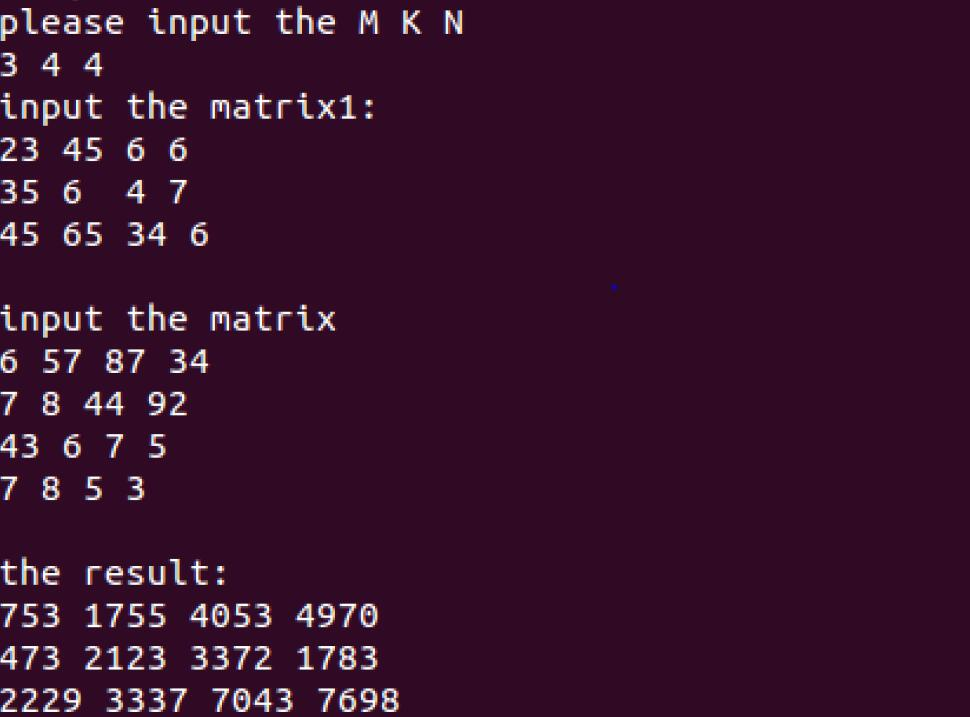
\includegraphics[scale= 0.4]{./fig/linux_result.jpg}
	\caption{Result on Linux}
	\label{fig::linux result}
\end{figure}

\subsubsection{Acceleration of different core}
When I'm working on this project, problems happen that I can hardly improve the acceleration with different numbers of threads. The problem occurs from the CPU cores I used is restricted, such that improvement with more threads is equally running on a single core.

\begin{minipage}{0.5\textwidth}
	\begin{figure}[H]
		\centering
		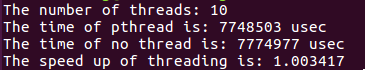
\includegraphics[scale= 0.8]{./fig/linux_result_core1.png}
		\caption{Accelerate with 1 core}
		\label{fig::linux with core1}
	\end{figure}
\end{minipage}
\begin{minipage}{0.5\textwidth}
	\begin{figure}[H]
		\centering
		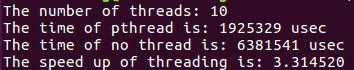
\includegraphics[scale= 0.8]{./fig/linux_result_core2.png}
		\caption{Accelerate with multi-cores}
		\label{fig::linux with core2}
	\end{figure}
\end{minipage}
\subsection{Windows}
\subsubsection{Result}
The Matrix Multiplication result on Windows is as follows:
\begin{figure}[H]
	\centering
	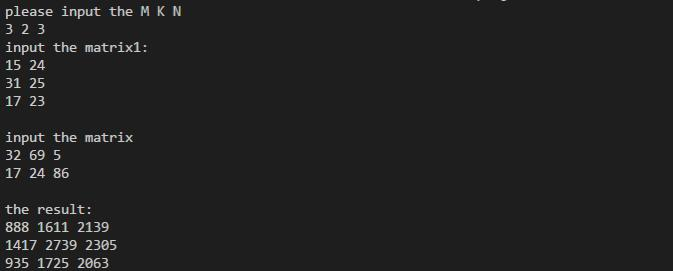
\includegraphics[scale= 0.5]{./fig/win_result.jpg}
	\caption{Result on Windows}
	\label{fig::result on windows}
\end{figure}
\subsubsection{Acceleration of different threads}\label{Part: Use different threads }
If we want to fully employ the acceleration, we must make relevant matrix large enough to avoid that creating pthread consumes too much time. Therefore, I choose $10$ and $100$ threads for a matrix whose size is $1000 \times 1000$.

\begin{minipage}{0.5\textwidth}
	\begin{figure}[H]
		\centering
		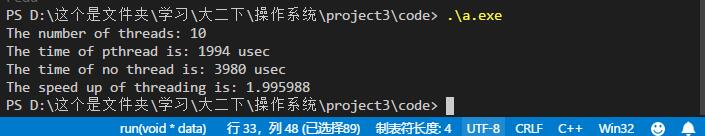
\includegraphics[scale= 0.45]{./fig/win_result_10.jpg}
		\caption{Accelerate with 10 threads}
		\label{fig::windows 10 threads}
	\end{figure}
\end{minipage}
\begin{minipage}{0.5\textwidth}
	\begin{figure}[H]
		\centering
		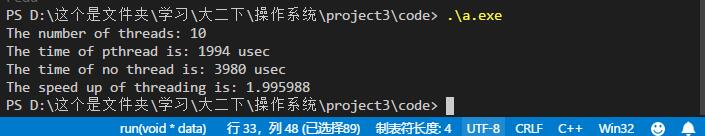
\includegraphics[scale= 0.45]{./fig/win_result_10.jpg}
		\caption{Accelerate with 100 threads}
		\label{fig::windows 100 threads}
	\end{figure}
\end{minipage}
\par \quad
\par
It is easy to see that in such condition, a relatively-more-threads methods trades off for a more ideal acceleration. But will more threads always result in better performance? And how will the size of the matrix affect the performance? We will discuss this at Part \ref{part::project analysis}.
\section{Project Analysis}\label{part::project analysis}

\subsection{Thread Mountain}
\begin{figure}[H]
	\centering
	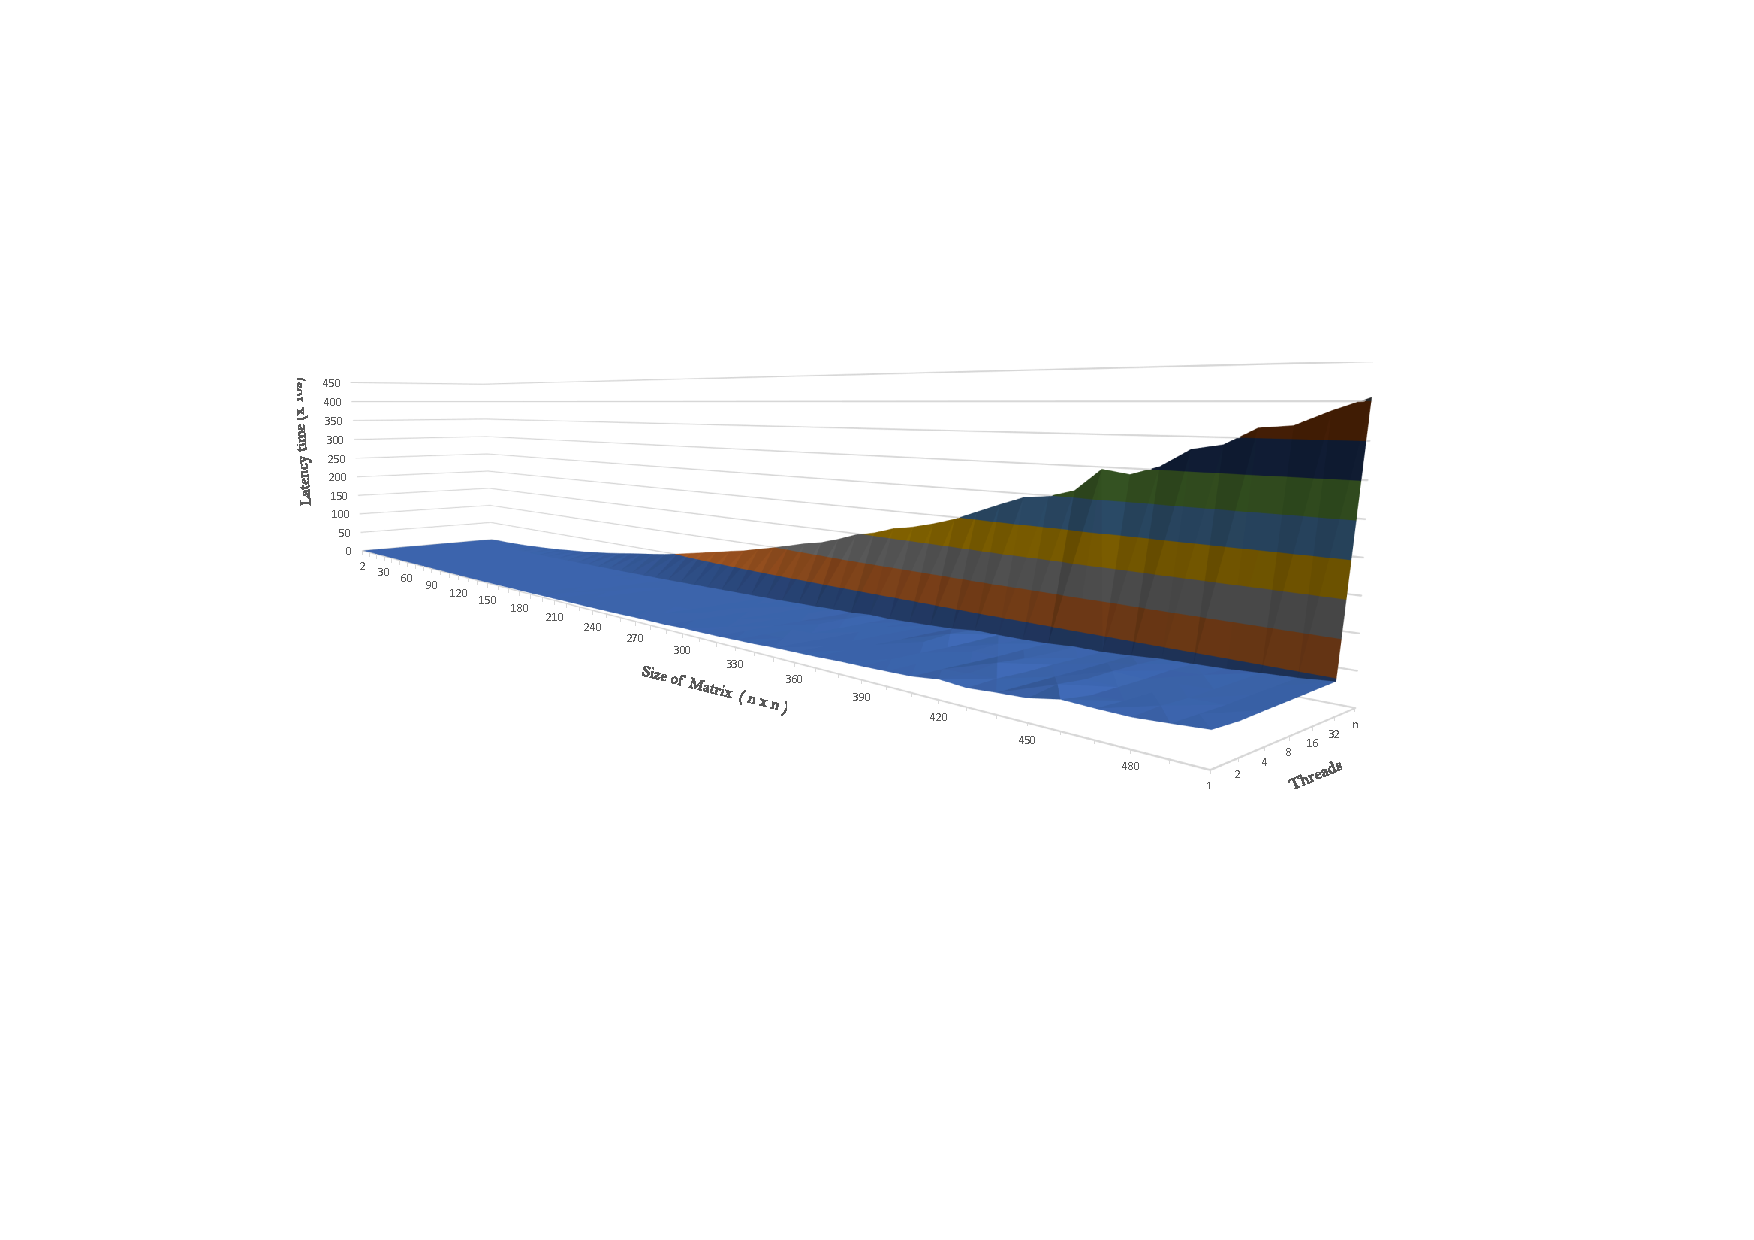
\includegraphics[scale= 0.7]{./fig/data_test.pdf}
	\caption{Thread Mountain}
	\label{fig::Thread Mountain}
\end{figure}

\quad  Similar to the idea from famous "Memory Mountain" introduce on <<Computer Systems: A Programmer's Perspective>>\cite{Bryant2015Computer}, I change the size of the matrix and the number of thread to examine how such things affect our performance.

If we continuously  run this program with different sizes and threads, then we can recover a fascinating two-dimensional function of running time versus size and threads, which I named it as \textbf{"Thread Mountain"} Figure \ref{fig::Thread Mountain}.

It is intuitive to see that $n\times n$ threads consumes much more time than others. So in the analysis follows, I change $n \times n$ threads into $n$ threads to make them under the same magnitude.

From a brief observation, we can easily conclude that more threads takes fewer time ( for the descending slope from $1$ to $32$ threads ). Considering small size matrices, $n\times n $ threads is not severely bad performed. However, at the turning point around $256\times 256$ (actual size $4$ KB in cache), its performance gets worse and worse for a deep cache miss.

Also, we can see small "Wrinkles" in the \textbf{Blue Parts} of this mountain, because our number is generated randomly, so it is normally to see small variance.
\subsection{Analysis of Thread Mountain}
\subsubsection{At the Foot of Thread Mountain}

\begin{figure}[H]
	\centering
	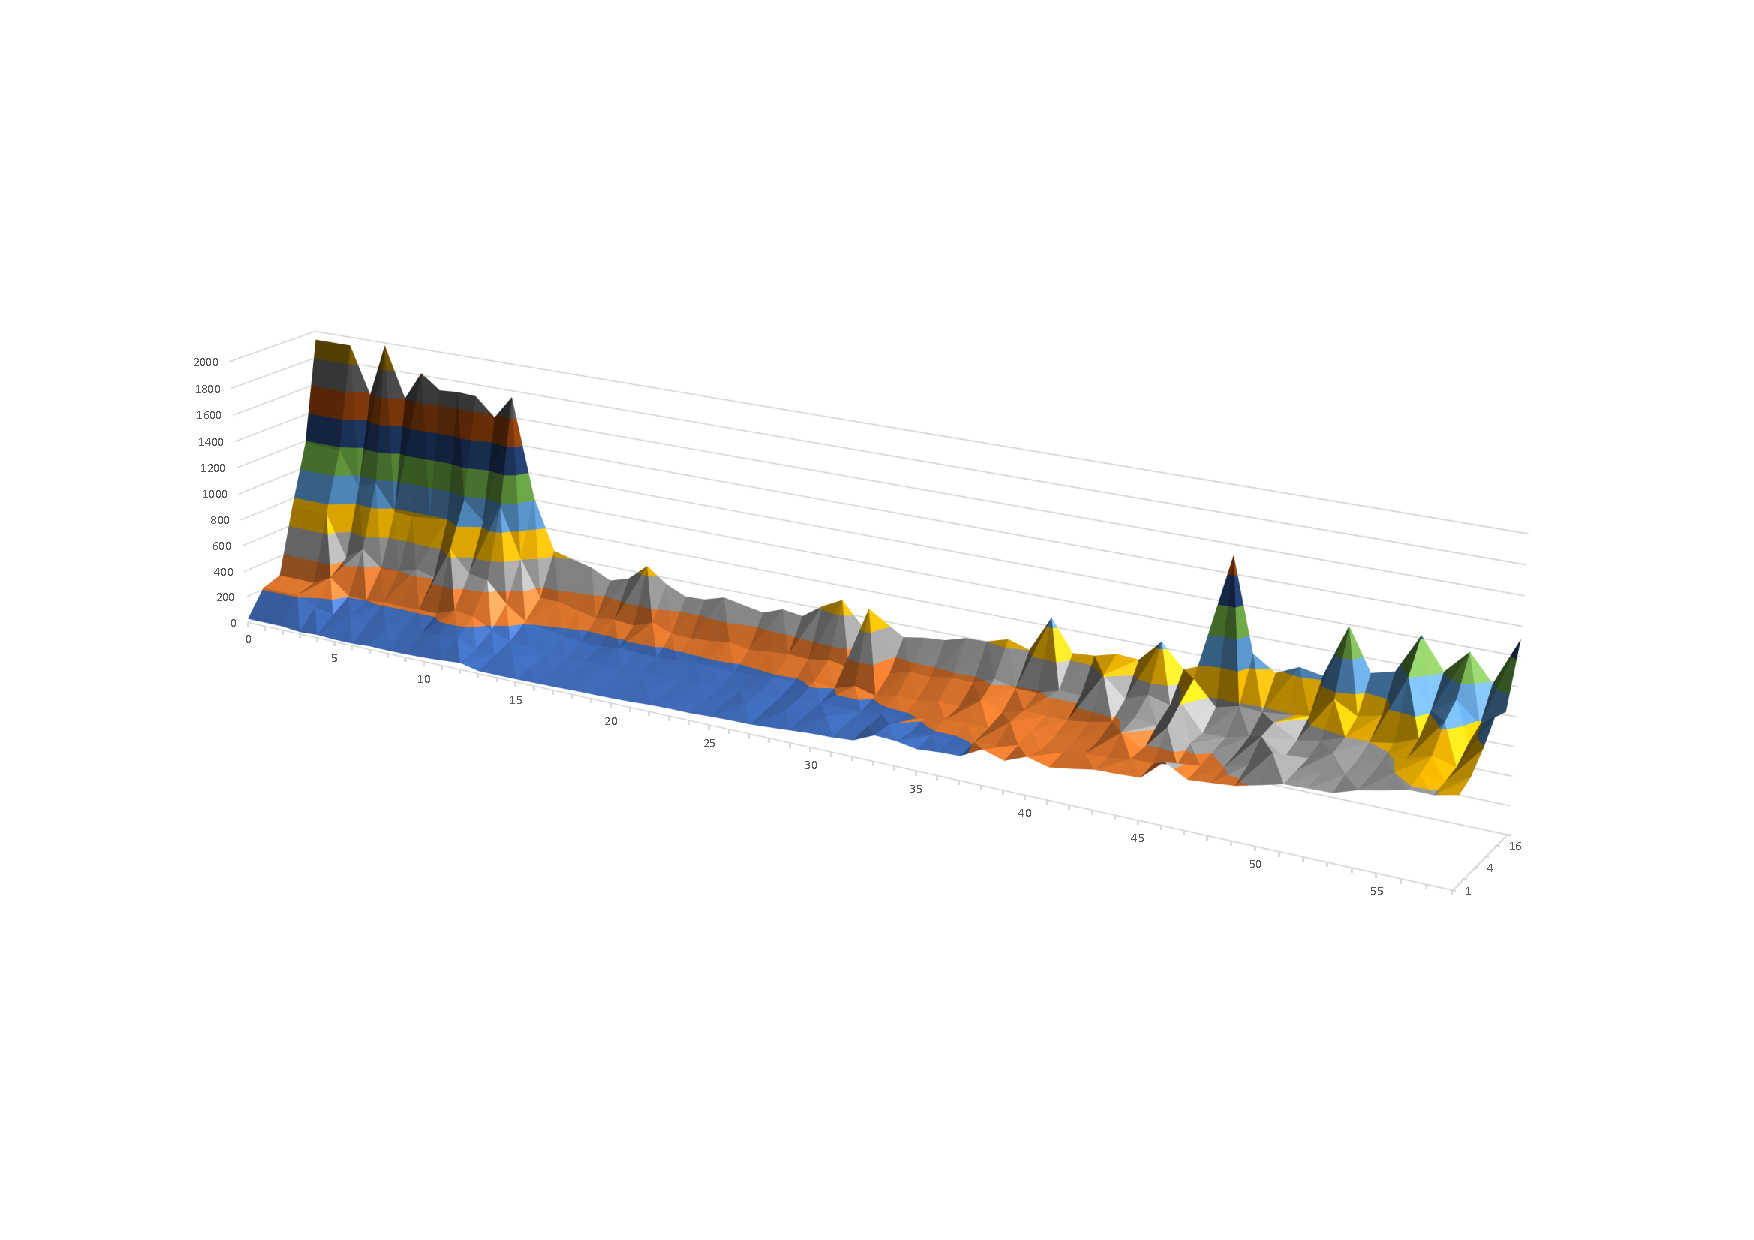
\includegraphics[scale= 0.65]{./fig/1_32_thread_0_50.pdf}
	\caption{The Bottom of Thread Mountain}
	\label{fig::bottom1 of thread mountain}
\end{figure}

When we focus on the bottom part of Thread Mountain, as is shown in Figure \ref{fig::bottom1 of thread mountain}, a strange phenomenon appears. We find that the starting part, from $1\times1$ to $10 \times 10$, consumes relatively 10 times of the following part. It is even longer than the matrix of $50\times 50$!

This can derive from what we called \textbf{Cold Miss} in our cache. After putting into L1 Cache, the time wasted on Cache Miss is much shorter. Besides, I think that when size is small, program will not be allocated much space in CPU according to relative optimization. When I open System Monitor, I find these program will be allocated much more space when getting larger as in Figure \ref{fig:: CPU Allocated}.


\begin{minipage}{0.4\textwidth}
	\begin{figure}[H]
		\centering
		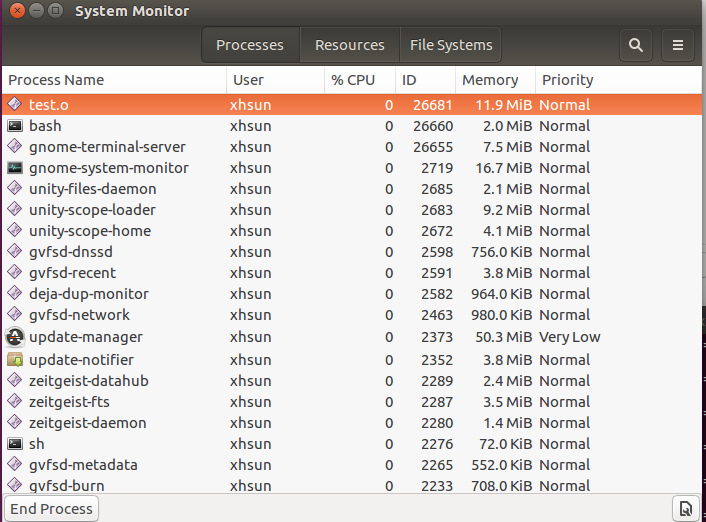
\includegraphics[width=0.7\textwidth]{./fig/Screenshot_0.png}
	\end{figure}
\end{minipage}
\begin{minipage}{0.4\textwidth}
	\begin{figure}[H]
		\centering
		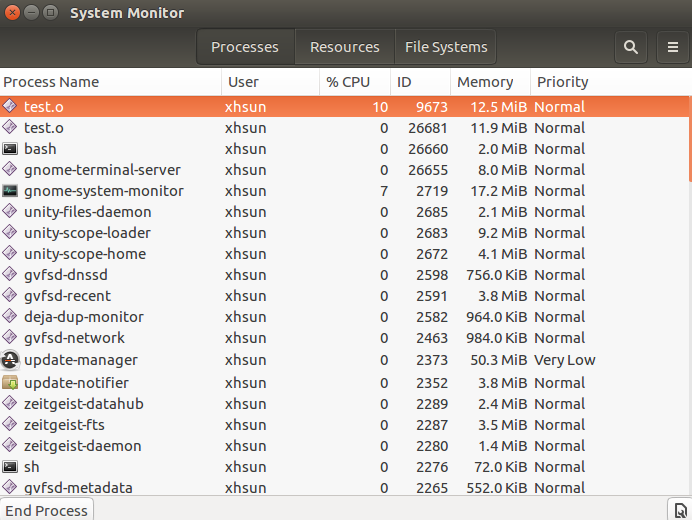
\includegraphics[width=0.7\textwidth]{./fig/Screenshot_10.png}
	\end{figure}
\end{minipage}

\begin{minipage}{0.4\textwidth}
	\begin{figure}[H]
		\centering
		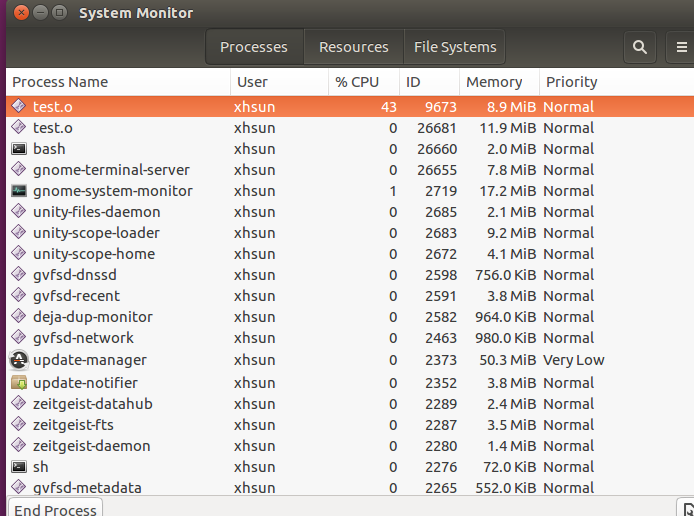
\includegraphics[width=0.7\textwidth]{./fig/Screenshot_43.png}
	\end{figure}
\end{minipage}
\begin{minipage}{0.4\textwidth}
	\begin{figure}[H]
		\centering
		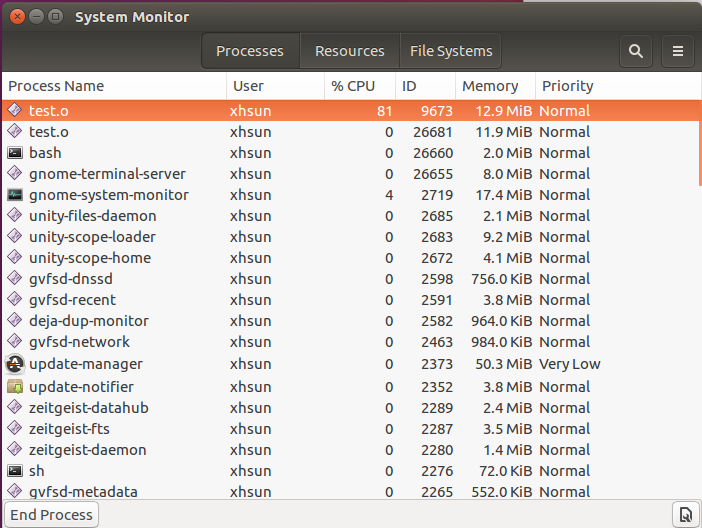
\includegraphics[width=0.7\textwidth]{./fig/Screenshot_81.png}
	\end{figure}
\end{minipage}
\begin{figure}[htbp]
	\centering
	\caption{CPU Allocated to this program growing from $0\%,10\%,43\%,81\% $}
	\label{fig:: CPU Allocated}
\end{figure}

From a Larger size varying from $1\times 1 $ to $90\times 90$, the time for single thread is fastest. There also exist several "Peaks" along the ridge, causing by difference of random number and the current CPU allocated to it.
Interestingly, in such case, until around $100\times 100$ multi-threads programming does not performs better, and the expense paid for creating new threads is too large.

\begin{figure}[H]
	\centering
	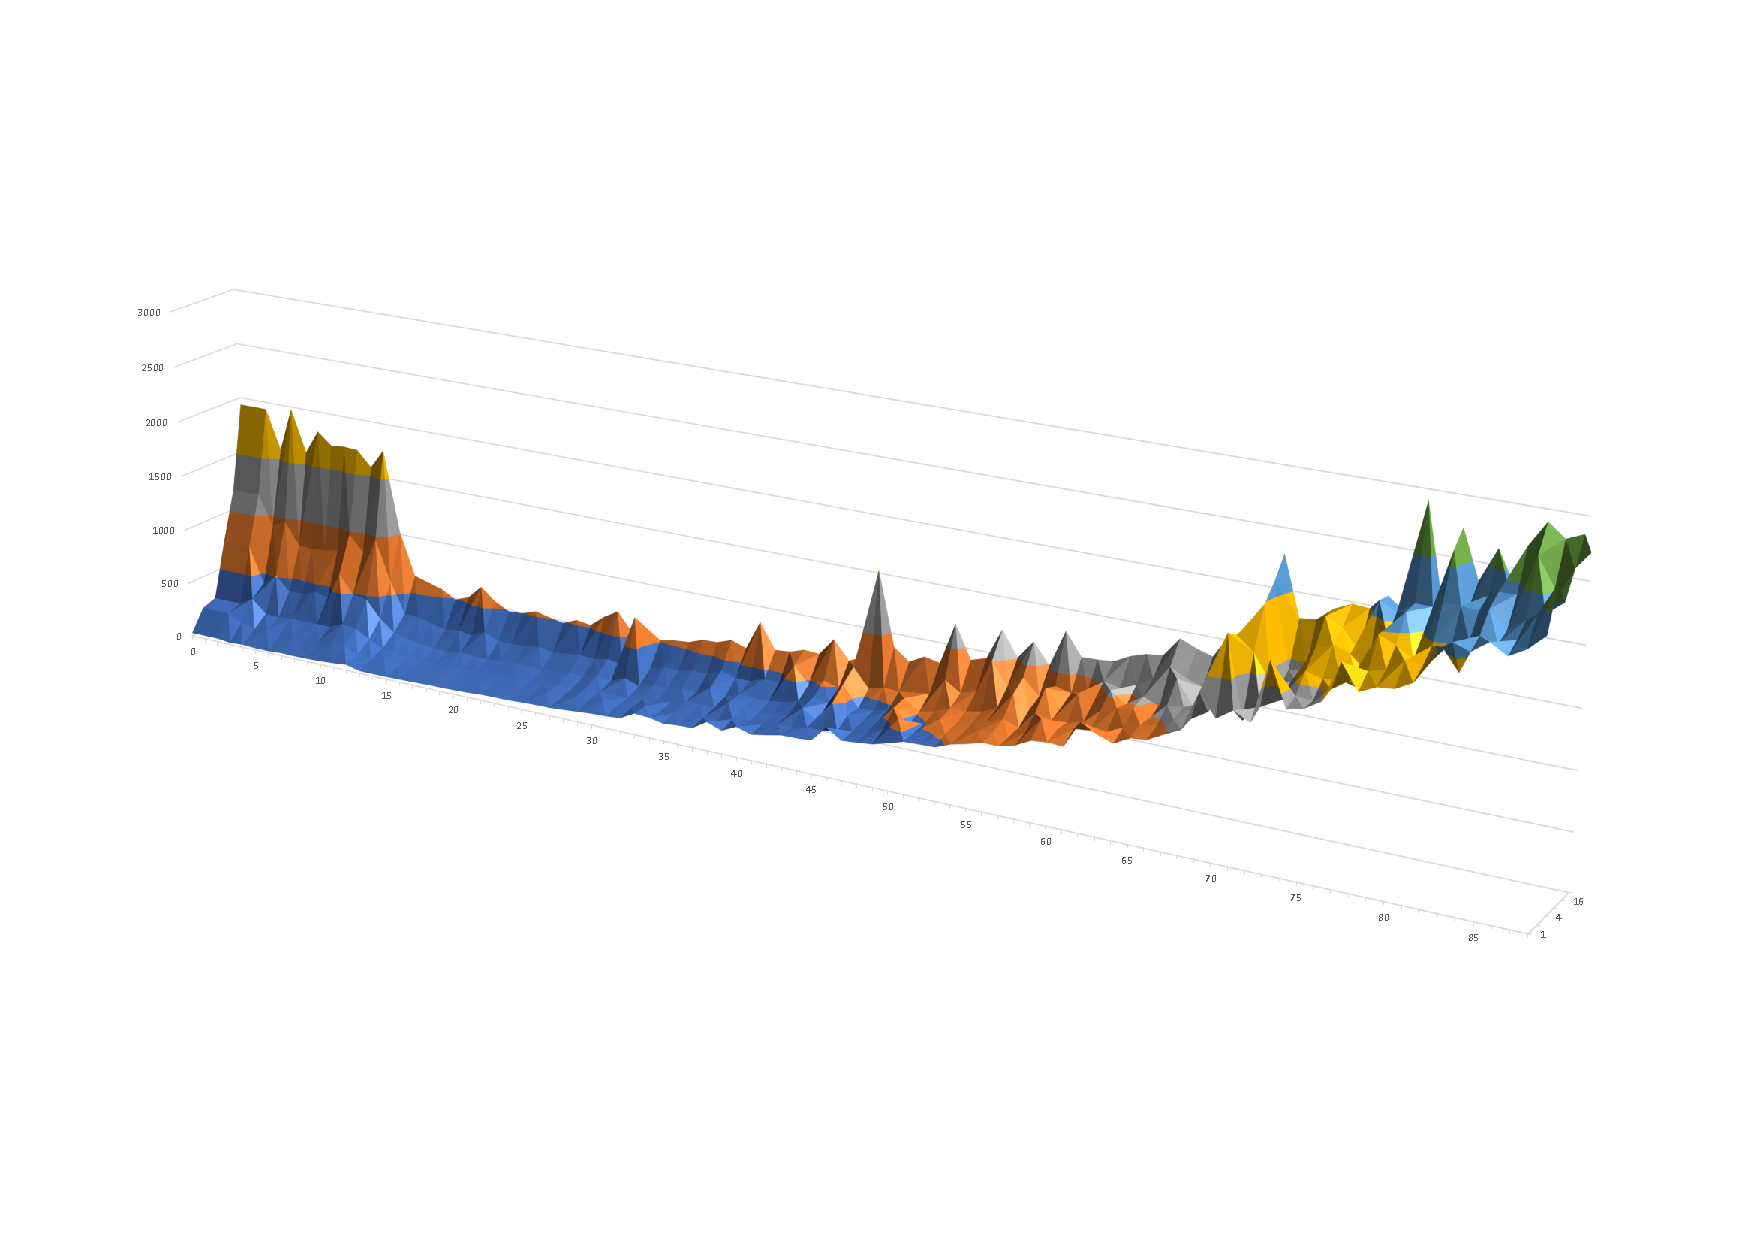
\includegraphics[scale= 0.75]{./fig/1_32_thread_0_90.pdf}
	\caption{A Larger Bottom of Thread Mountain}
	\label{fig::bottom2 of thread mountain}
\end{figure}

Hence, when we need to conduct operations on some small matrices, we can use single threads as an optimal solution. And here we shall try our best to eliminate the side effects from the "Cold Start" by earlier warm-up before executing our programs.

\subsubsection{Sharp Dips of the Throughput: Difference in Threads}\label{Part: Sharp Dips of Throughput}
This part we discuss the relation of different threads, and use \textbf{Throughput} to measure their behaviour.

At small size, different threads do not appear much difference. After about $75$, the First Dip comes out between $2$ threads and $4$ threads with throughput double. The corresponding acceleration rate is about $37\%$-$72\%$. After about $110$, the Second Dips between $32$ threads and $n$ threads, speeding up about $50\%$-$82\%$.

\begin{figure}[H]
	\centering
	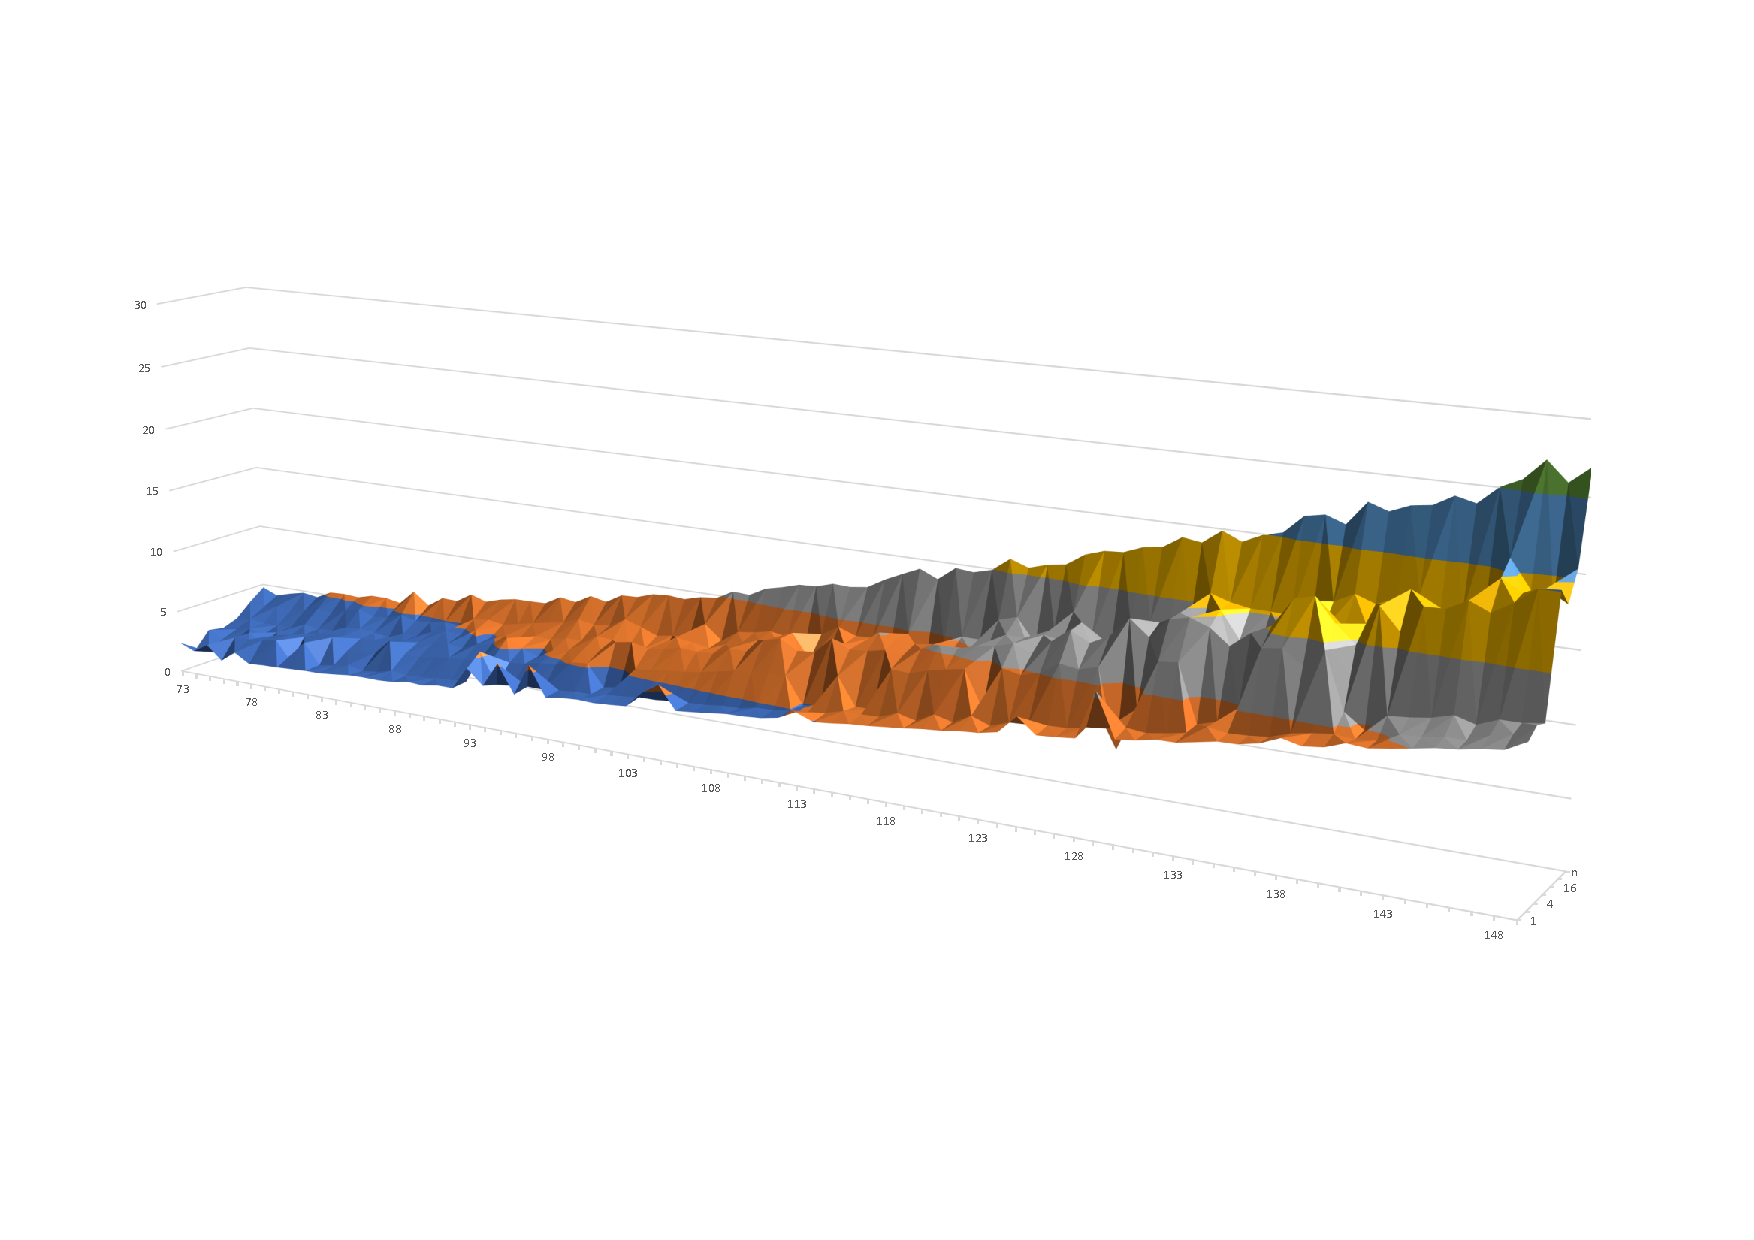
\includegraphics[scale= 0.6]{./fig/1_n_thread_73-140.pdf}
	\caption{Throughput of $1,2,4,8,16,32,n$ threads from size $70$ to size $150$}
	\label{fig::Throughput of 73-140}
\end{figure}

Things get different when size turns larger. Dips between $4$ threads and $8$ threads extend extremely large, then here is a platform between $8$ to $32$, and a small relative small dip between $32$ and $n$. This means that the difference on performance varies much among $4$ and $8$, probably because of the constraint of cache's size. And we can see the trade off between calculating new matrix and creating new threads is fairly acceptable. But when the matrix grows too large, e.g. $\geq300$ as in Figure \ref{fig::Throughput of 300-500}  because $n$ will get too large, so the corresponding creating and scheduling so much threads in CPU consume unbearable time and space.

\begin{minipage}{0.5\textwidth}
	\begin{figure}[H]
		\centering
		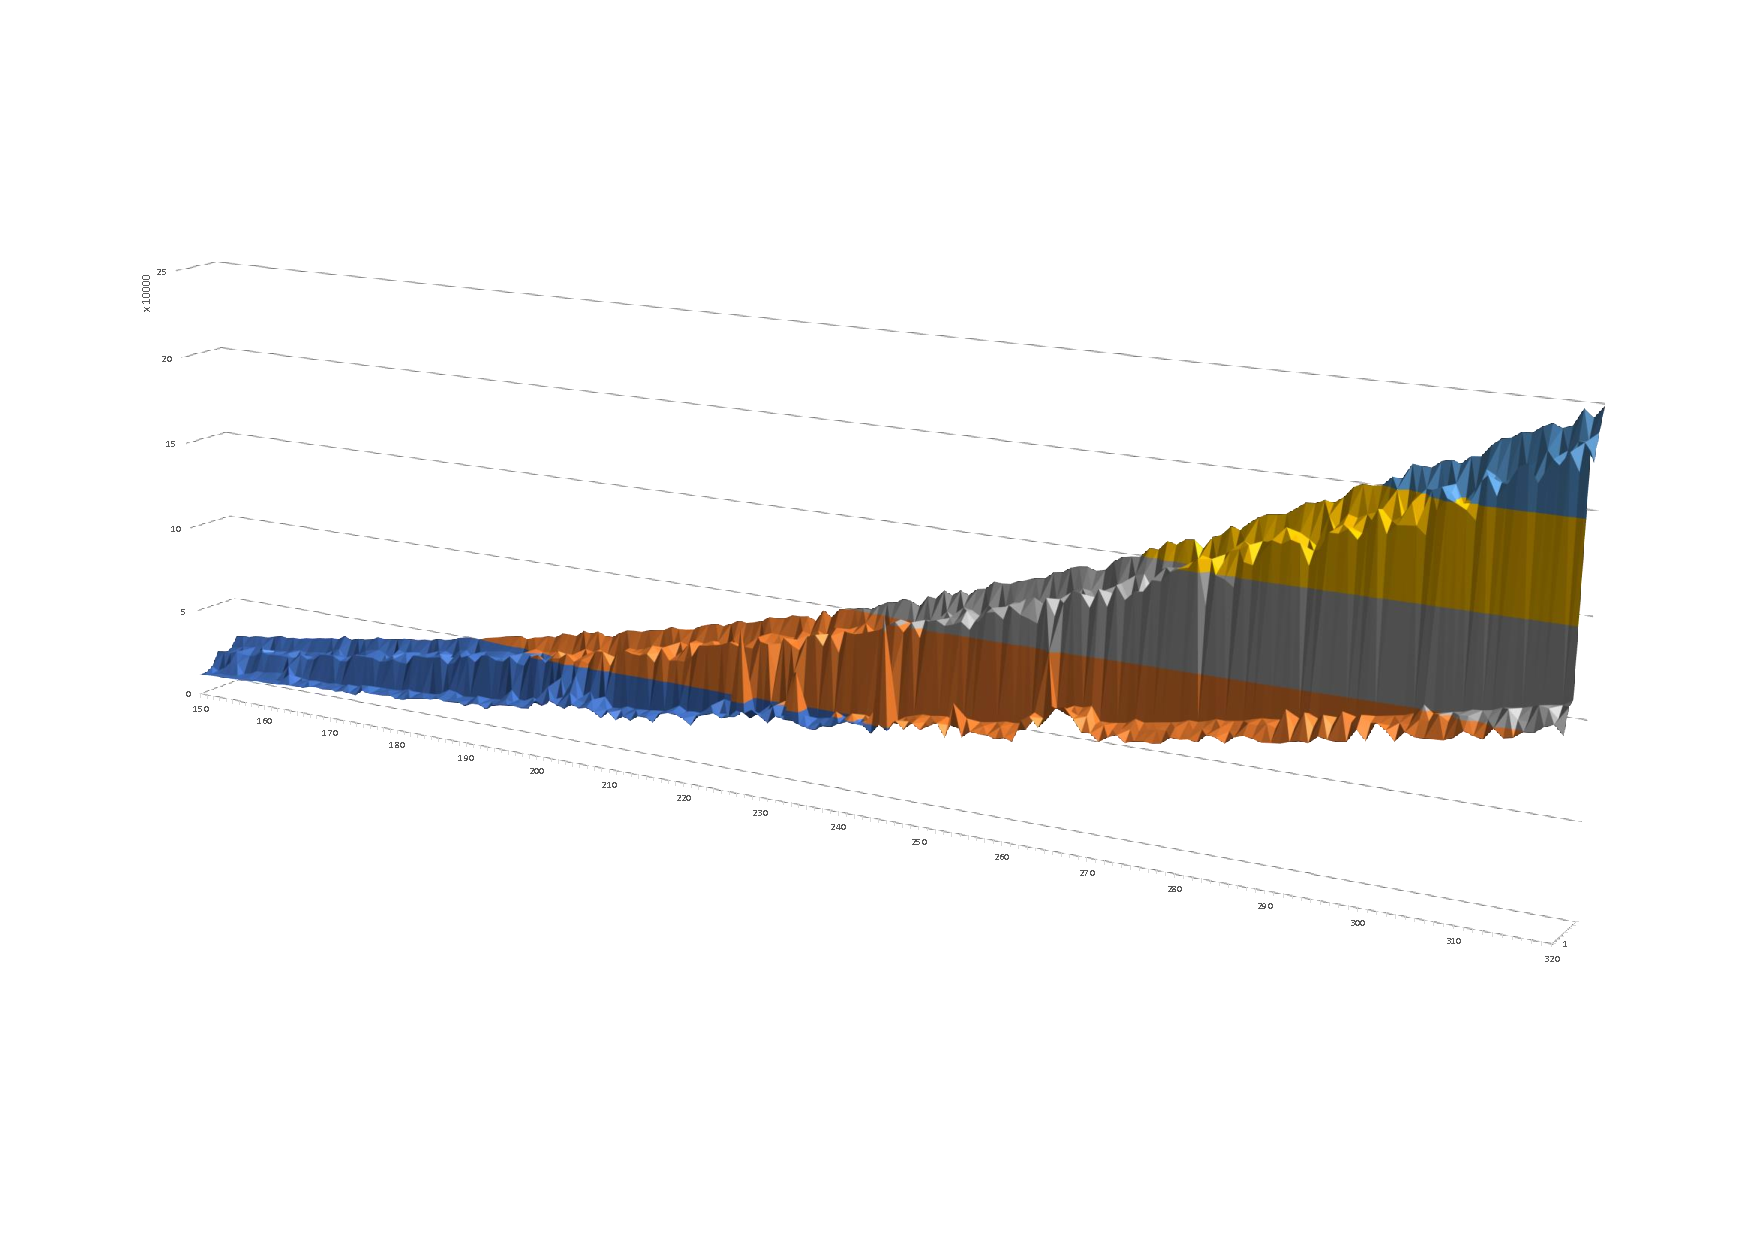
\includegraphics[width=0.85\textwidth]{./fig/1_n_thread_150-320.pdf}
		\caption{Throughput  from size $150$ to size $320$}
		\label{fig::Throughput of 150-320}
	\end{figure}
\end{minipage}
\begin{minipage}{0.5\textwidth}
	\begin{figure}[H]
		\centering
		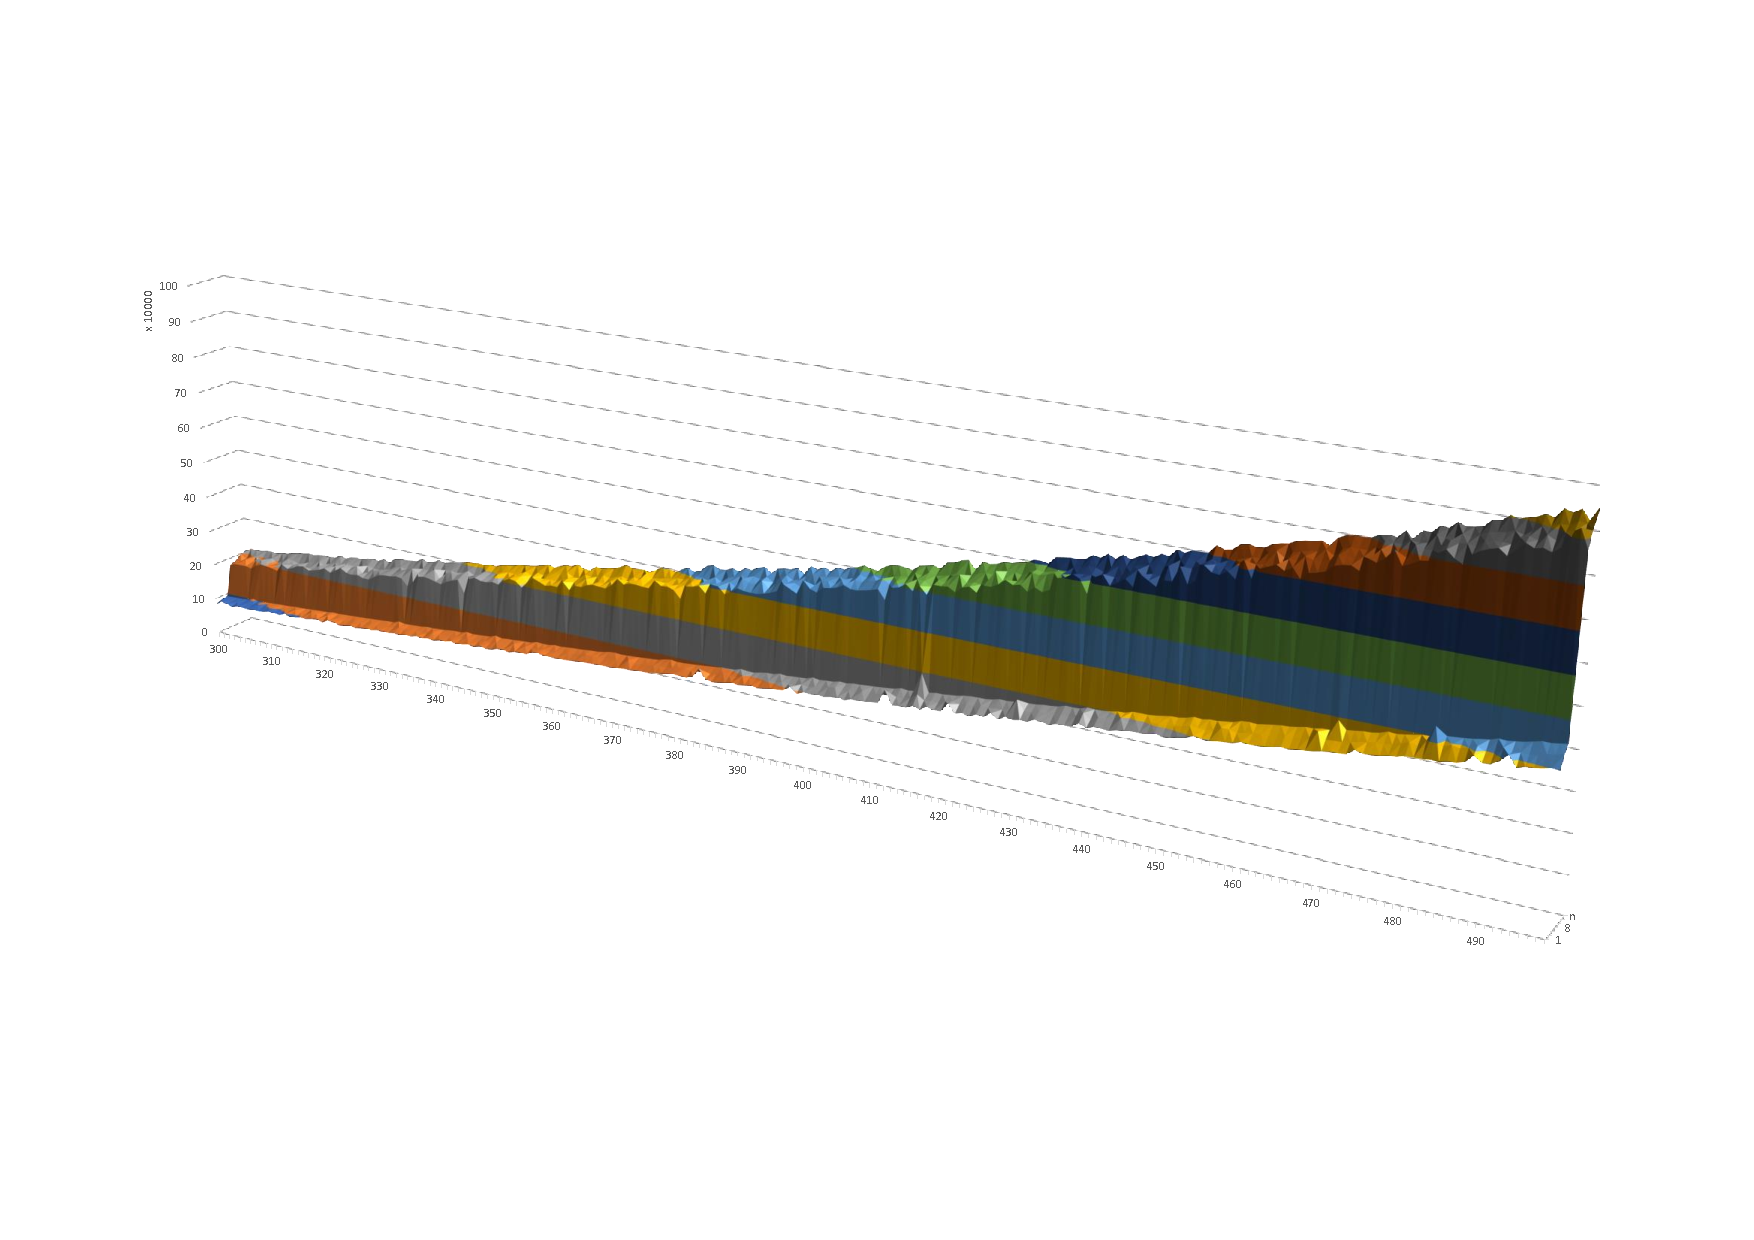
\includegraphics[width=0.85\textwidth]{./fig/1_n_thread_300-500.pdf}
		\caption{Throughput from size $300$ to size $500$}
		\label{fig::Throughput of 300-500}
	\end{figure}
\end{minipage}

When viewing from a higher perspective, the difference between $4$ and $8$ threads gets more severe, and other differences become not that obvious. Besides, as is shown in Figure \ref{fig::Throughput of 500-700}, the \textbf{Robustness} for multi-threads programming is better, for the wrinkles change severe on $1,2,4$-threads programming but remain almost unchanged on $4$~$n$-threads programming.

\begin{figure}[H]
	\centering
	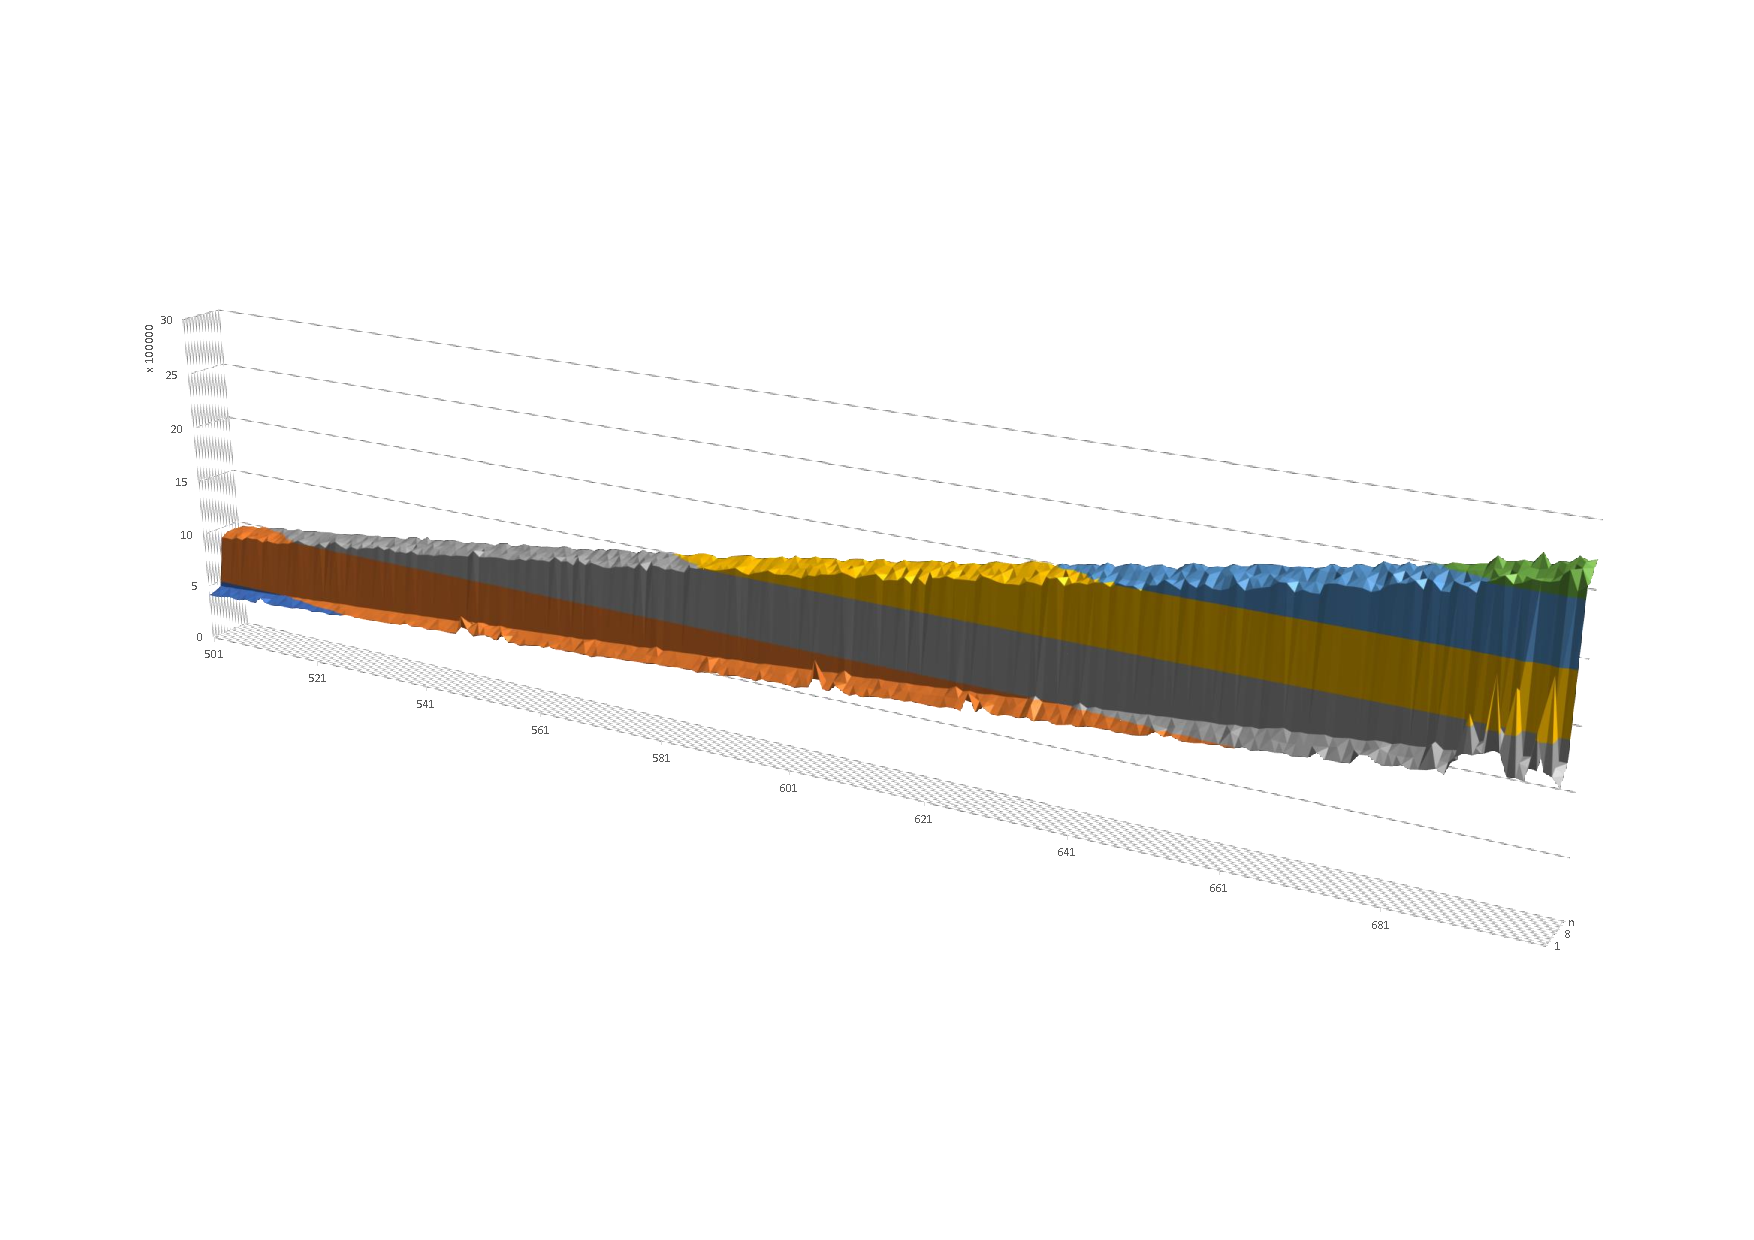
\includegraphics[scale= 0.65]{./fig/1_n_thread_500-700.pdf}
	\caption{Throughput from size $500$ to size $700$}
	\label{fig::Throughput of 500-700}
\end{figure}

\subsubsection{Ridge Line}
When consider a special number of threads, e.g. $2$ as is shown in Figure \ref{fig::ridge line of 90-150} and Figure \ref{fig::ridge line of 300-500}, the trends for this goes approximately up with small wrinkles somewhere.

When the size is small, e.g. $90$ to $150$ in Figure \ref{fig::ridge line of 90-150}, wrinkles not vary much. Using Matlab, the variance in performance is restricted in $28.7$.

As size goes larger, e.g. $300$ to $500$ in Figure \ref{fig::ridge line of 300-500}, wrinkles vary fairly much. The larger the size goes, the worse the variance becomes. At around $460$ the variance is up to $174.3$. The average for $300$-$500$ is about $1.76$ times of $90$-$150$.

\begin{minipage}{0.5\textwidth}
	\begin{figure}[H]
		\centering
		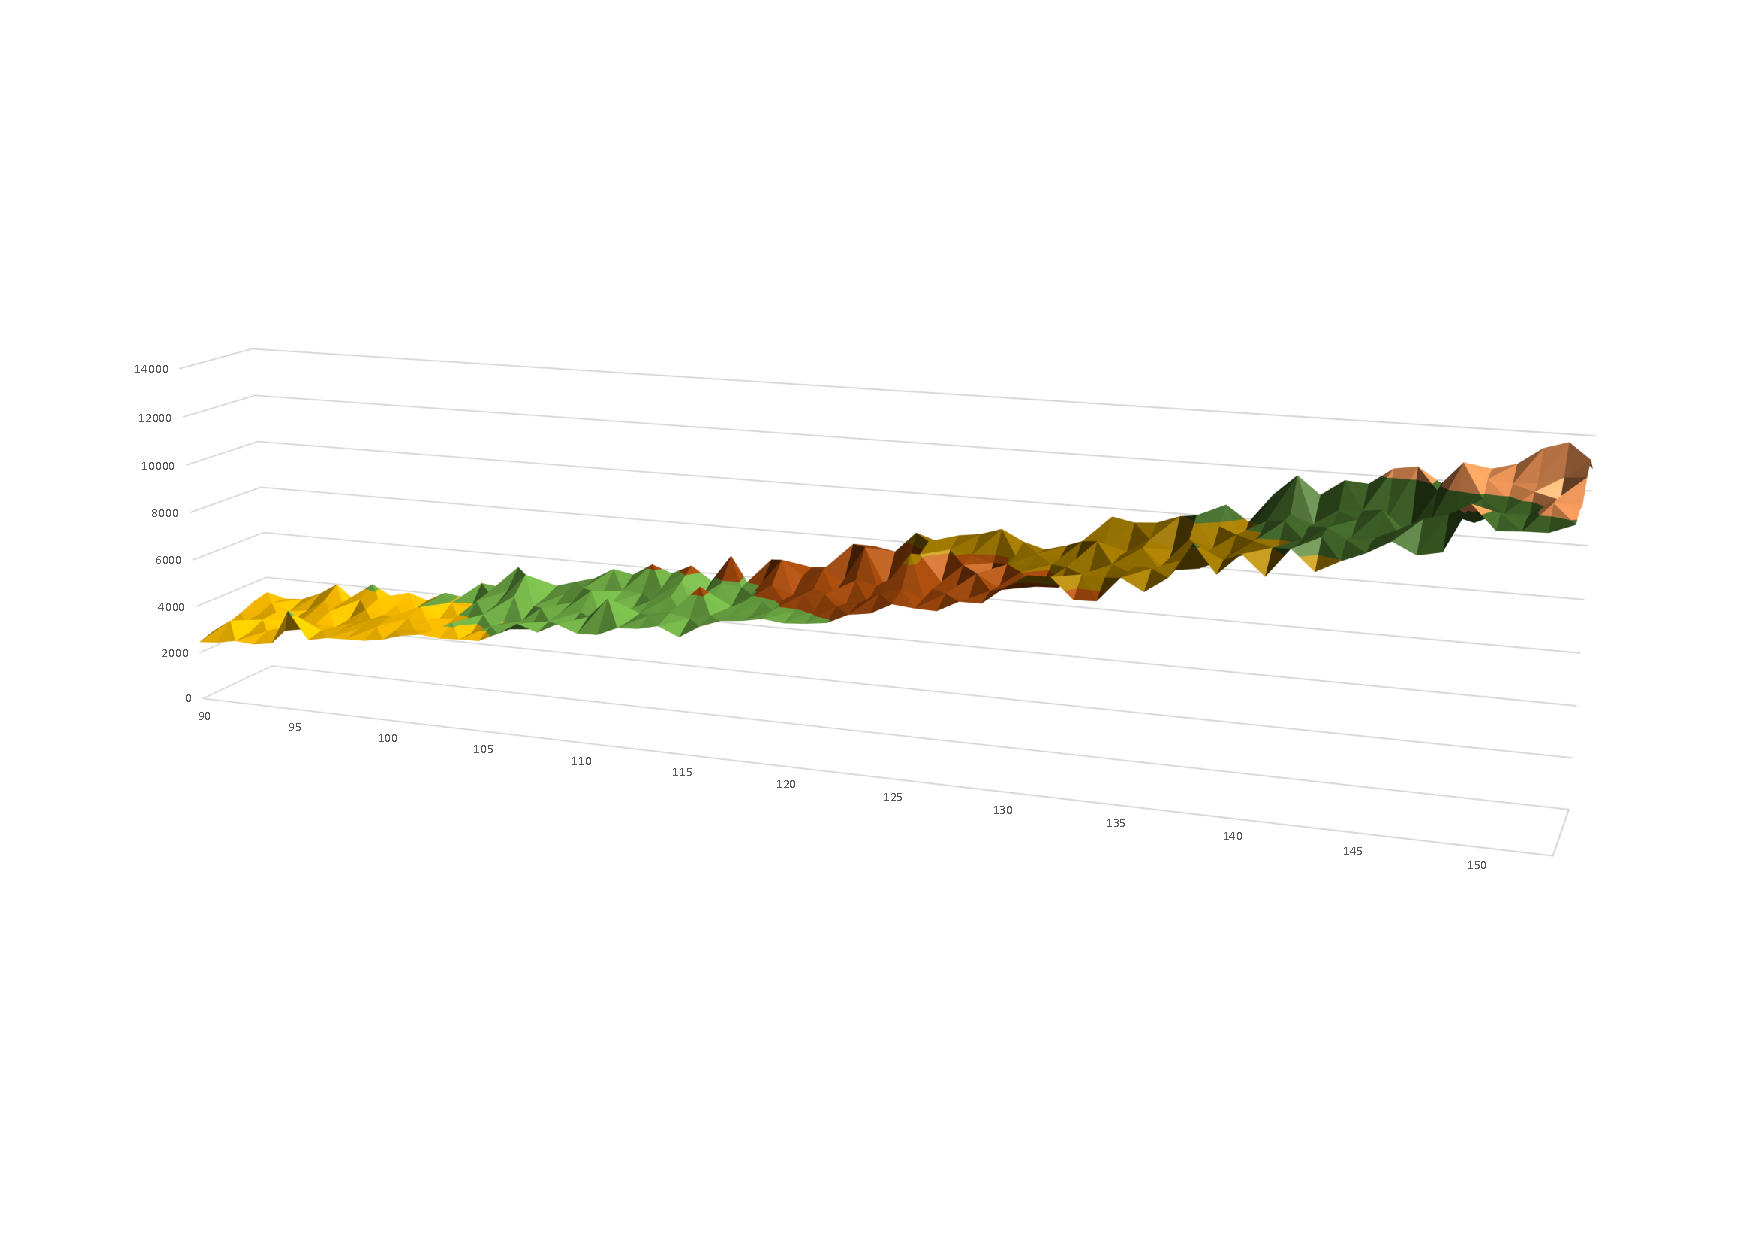
\includegraphics[width=0.97\textwidth]{./fig/ridge_1.pdf}
		\caption{Ridge Line From $90$ to $150$}
		\label{fig::ridge line of 90-150}
	\end{figure}
\end{minipage}
\begin{minipage}{0.5\textwidth}
	\begin{figure}[H]
		\centering
		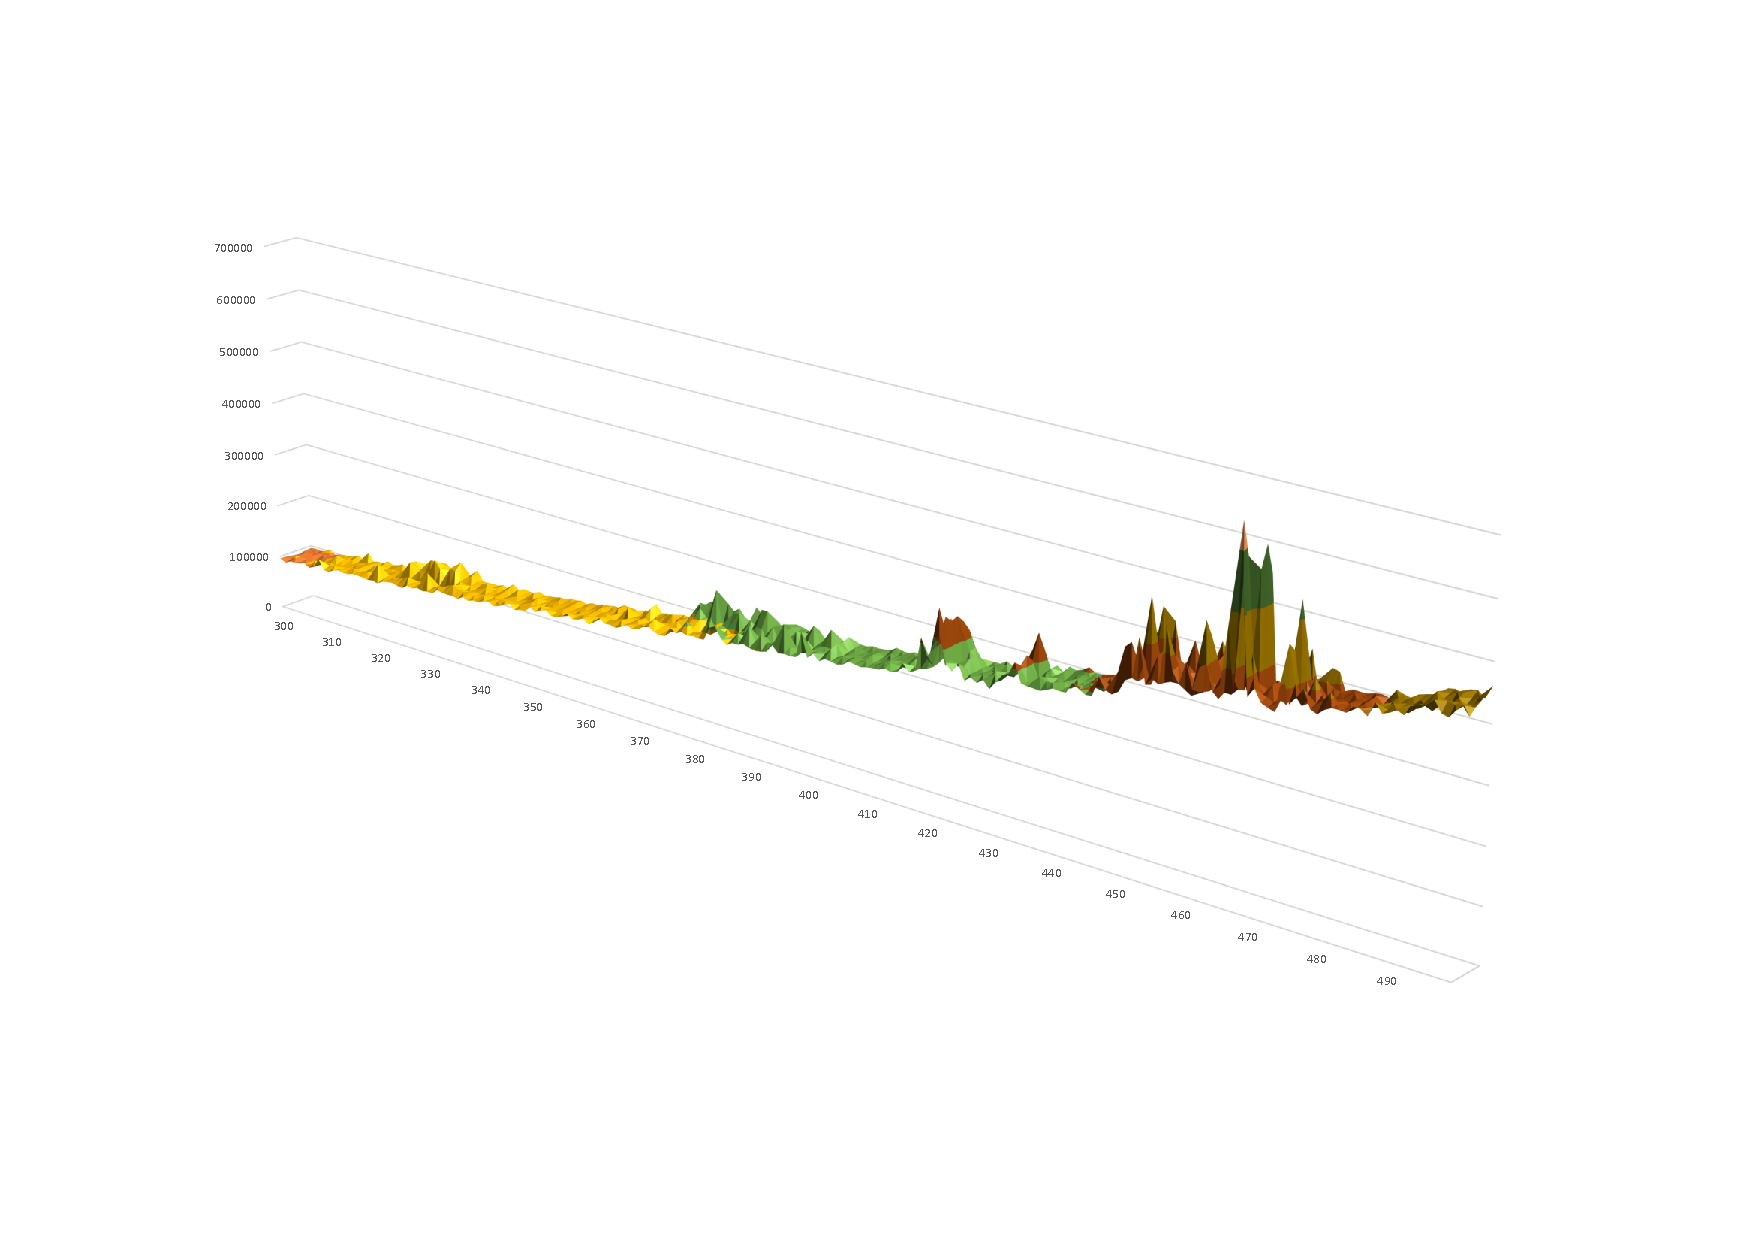
\includegraphics[width=0.65\textwidth]{./fig/ridge_2.pdf}
		\caption{Ridge Line From $300$ to $500$}
		\label{fig::ridge line of 300-500}
	\end{figure}
\end{minipage}

\subsection{$n \times n $ Threads Performance}
If we take a slice though the mountain, holding the stride constant as in Figure \ref{fig::Thread Mountain}, we can see the impact of size on $n\times n $ threads. Since we create too many threads, its time latency can be badly frustrating. View from Figure \ref{fig::n x n threads time latency}, it is interesting to see two sharp dips at around size $2^6=64$ and $2^8=256$.

Such dips occur may result from the size constrained by the cache. Besides, around the platform and the edges, there appear some small drops but not violating the magnitude. This may result from conflicts with code and data lines, especially in such a busy program where threads' instructions interact with matrix data quite often.

\begin{figure}[H]
	\centering
	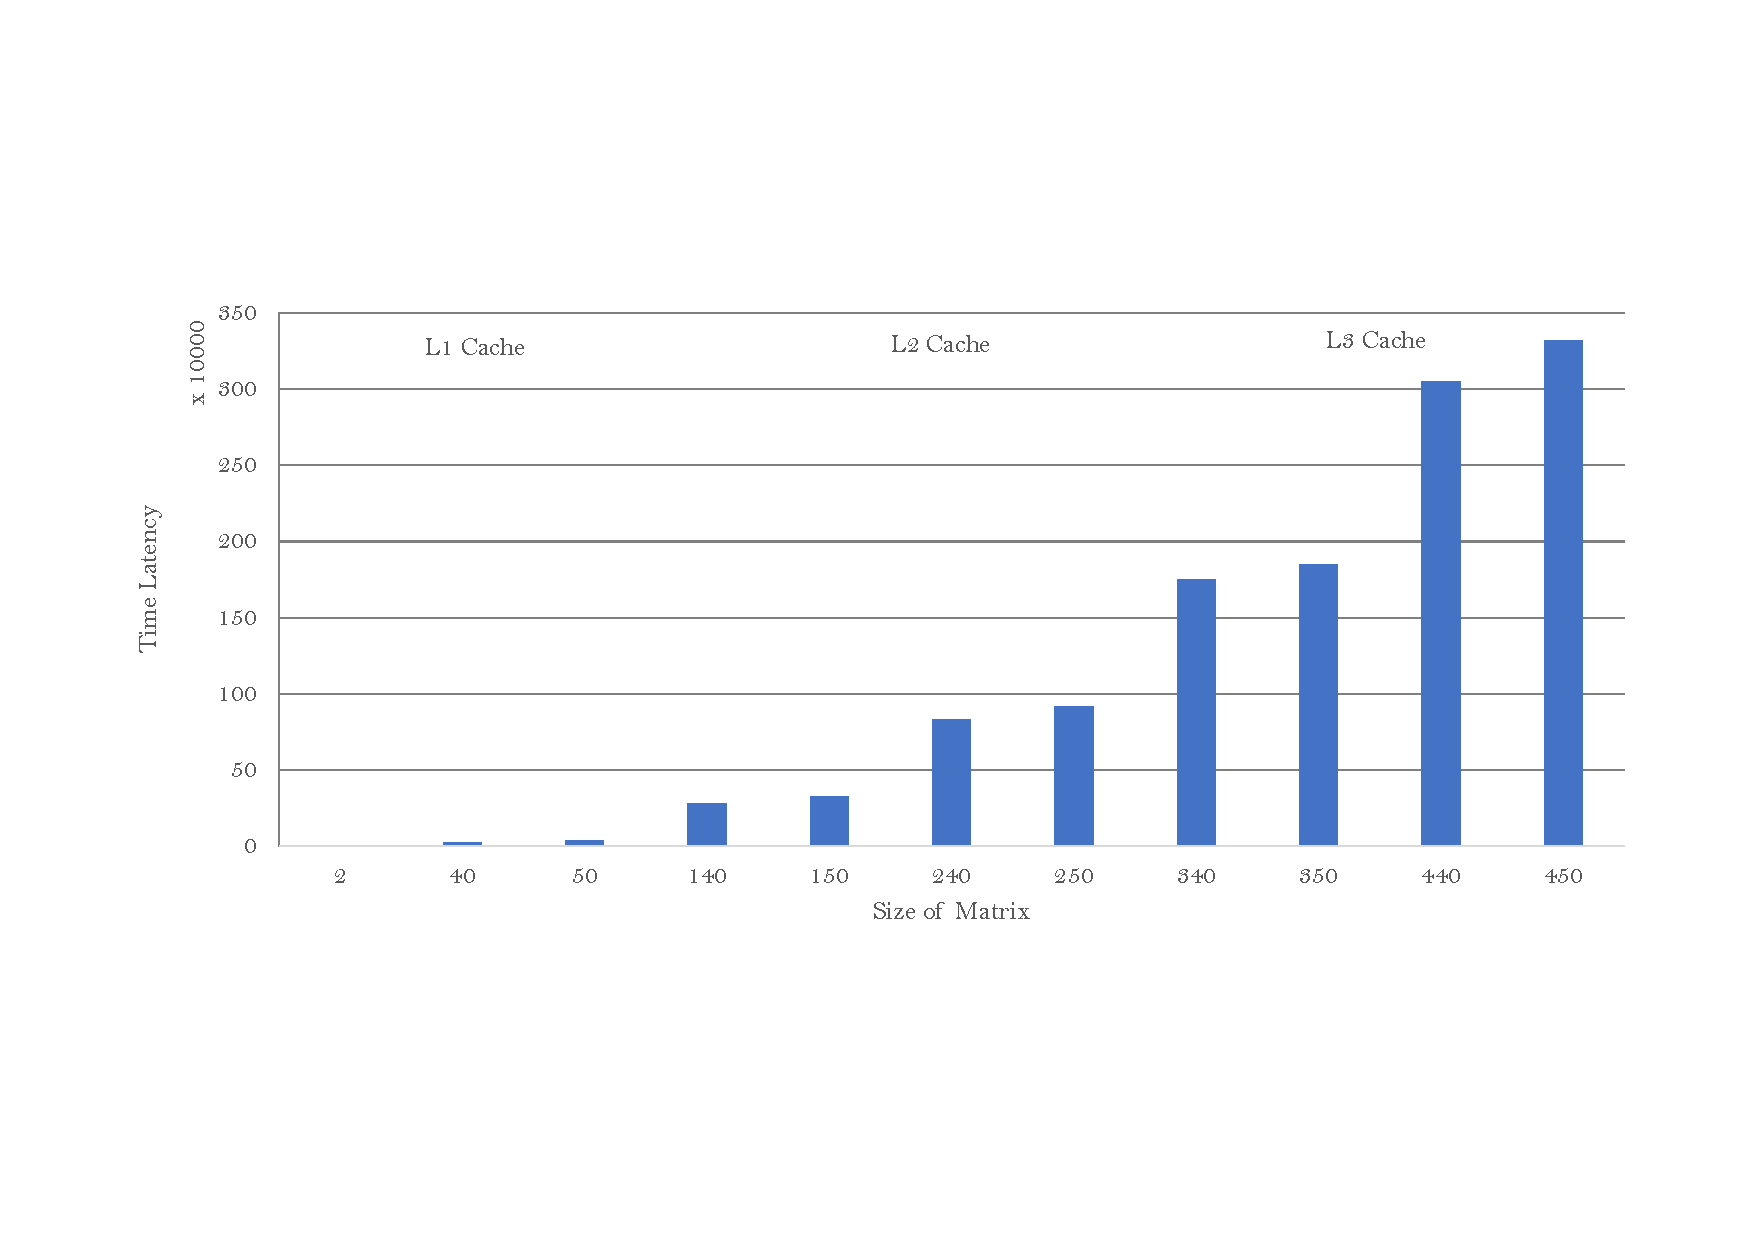
\includegraphics[scale= 0.6]{./fig/n_thread_chart.pdf}
	\caption{$n\times n $ Time Latency}
	\label{fig::n x n threads time latency}
\end{figure}


\section{Problems Conquered}
\subsection{Pid is the Same}\label{Part:Pid is the same}
\begin{minipage}{0.5\textwidth}
	In my very first attempt, I output my Pid but all threads' id is the same, which means I didn't actually use parallel programming at all.

	\quad After searching on Google, I find my \textbf{Threadjoin()} function comes exactly after each \textbf{CreateThread()} function. This means, every time I create a thread I exactly create it and wait for its end, but not create many threads, running them concurrently and end them at the same time.

	\quad Interestingly enough, when on Virtual Box, up-speeding is much faster than on dual-systems. The reason may be different version of Ubuntu, one is 14.04 and another is 16.04. Corresponding optimization is continuously improved.
\end{minipage}
\begin{minipage}{0.5\textwidth}
	\begin{figure}[H]
		\centering
		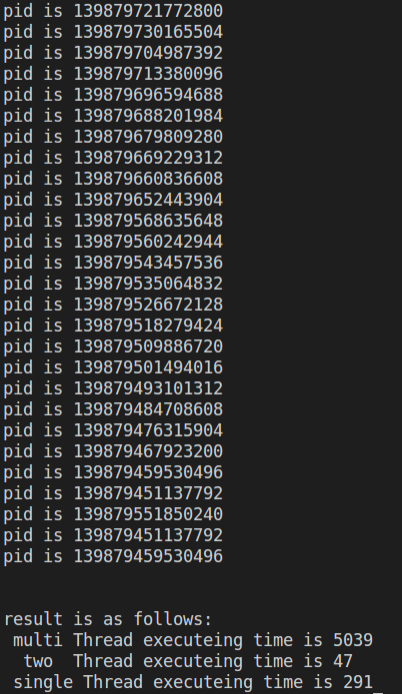
\includegraphics[width= 0.6\textwidth]{./fig/pid.png}
		\caption{Different Pid Under Multi-Threads Programming}
		\label{fig::pid}
	\end{figure}
\end{minipage}
\subsection{CPU Dumped Encountered with too Much Threads}
When running simulation for Part\ref{part::project analysis}, my CPU always dumped when the matrix is too large. As I take a closer look into this, I find that when encountered with $n\times n$ threads, this will consume too much space allocated to it. So I change it into several parts and use \textbf{Divide and Conquer} methods to complete the simulation.

\subsection{Running with Multi-Core}
During the process of writing my report, I running my code on Virtual Box on my Windows instead of dual-boot operating systems to make it easier for me to compare it with my previous results. But although the program runs with pretty satisfying acceleration rate on Linux, it fails to accelerate on Virtual Box.

This result is annoying but strange, after I call the system performance monitor, I find my CPU is always fully employed. So I instantly think whether on Virtual Box I have not use multi-cores, the result is obvious as Figure \ref{fig::multi-core} shows.

\begin{figure}[H]
	\centering
	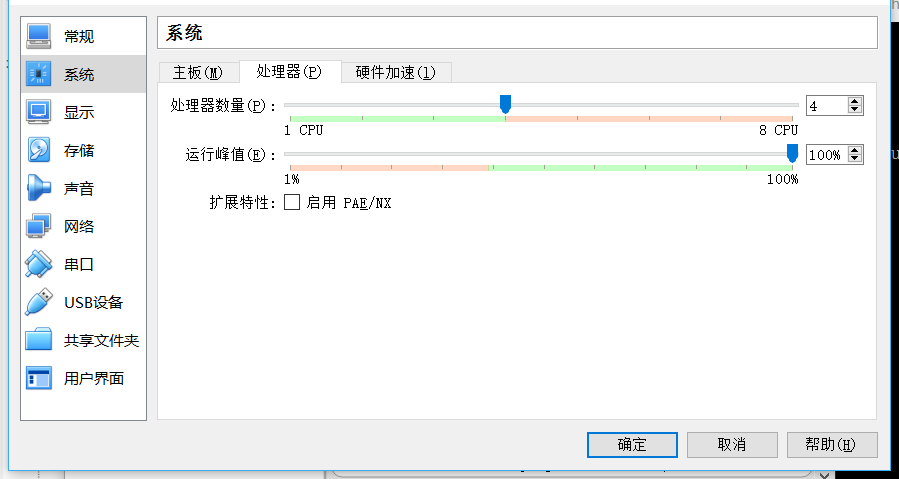
\includegraphics[scale= 0.4]{./fig/setting.png}
	\caption{Setting Virtual Box with Multi-Core}
	\label{fig::multi-core}
\end{figure}
\section{Harvest}

In this project, I have harvested pretty much. This project is easy to complete, but fully understanding it is another thing. By referring to what I have learned on Computer Architecture.
\begin{enumerate}
	\item \textbf{A better understanding of multi-thread programming and its completion.} I used to write several multi-thread python crawlers with "Threading" library. Corresponding principles are similar but varies on details, such that I make a better progress on multi-thread programming.
	\item \textbf{A better understanding of CPU and Threads.} As I have shown in Part \ref{part::project analysis}, after creating and analysing such a "Thread Mountain" helps me better to make sense of CPU and its performance. With methods similar to CSAPP, I find such a mountain is quite intuitive and straightforward.
	\item \textbf{A better understanding of Virtual Box compared with Dual-Boot Operating Systems.} The optimization used on Virtual Box reduces relevant performance to make two operating system can run at the same time.
\end{enumerate}

\section{Further Work}
Here is some Further Work which I feel needs a try:
\begin{enumerate}
	\item As is known, CPU may not be the best choice for Matrix Multiplication, so the performance on GPU and TPU is fascinating.
	\item I have not explore the scheduling of CPU, so there is a chance that because of other programs running at the same time, my simulation Thread Mountain is influenced without my awareness. So how to make the CPU unchanged during my simulation may need further exploration.
	\item The difference for threads programming on Windows and Linux is not clear, so maybe some tutorials can help figure out this and reconsider relevant performance on these two Operating Systems.
\end{enumerate}


\bibliographystyle{plain}
\bibliography{reference}
\end{document}
